% OpenCaseLaw — Paper 1 (Resource).
% Split from the v3 monolithic draft on 2026-05-21; fundamentally revised
% 2026-07-31 on the 2026-07-30 snapshot: corpus crossed 1M decisions, the
% resolver gained the oracle_xref stratum (93.8% coverage), three
% interpretive layers were added (scholarship bridge, administrative
% practice, expanded Botschaft links), and the deployed MCP surface now has
% measured agent adoption. The evaluation/audit content remains Paper 2
% scope. All headline numbers regenerate via scripts/paper_snapshot_stats.py
% against the serving databases; tables via v3/scripts/build_tables.py.
\documentclass[11pt,a4paper]{article}

\usepackage[T1]{fontenc}
\usepackage{lmodern}
\usepackage{textcomp}
\usepackage[margin=2.5cm]{geometry}
\usepackage[expansion=false,protrusion=false]{microtype}
\usepackage{xcolor}
\usepackage{xurl}
\usepackage[numbers,sort&compress]{natbib}
\usepackage[hidelinks,breaklinks=true]{hyperref}
\emergencystretch=2em
\usepackage{booktabs}
\usepackage{array}
\usepackage{graphicx}
\usepackage{float}
\usepackage{amsmath,amssymb}
\usepackage{authblk}
\usepackage[section]{placeins}
\usepackage{tikz}
\usetikzlibrary{positioning,arrows.meta,fit,backgrounds}
\newcolumntype{L}[1]{>{\raggedright\arraybackslash}p{#1}}
\setlength{\intextsep}{22pt plus 2pt minus 2pt}
\setlength{\textfloatsep}{22pt plus 2pt minus 4pt}
\setlength{\abovecaptionskip}{12pt}
\setlength{\belowcaptionskip}{6pt}

\title{OpenCaseLaw: A Verifiable Multilingual Research Substrate for Swiss Jurisprudence}

\author{%
  Jonas Hertner \\
  OpenCaseLaw \\
  \texttt{jh@jonashertner.com}
}

\begin{document}
\maketitle

\begin{abstract}
We release \textbf{OpenCaseLaw}, an open, verifiable research substrate for Swiss law: a resolved cross-court citation graph joined to several components of Swiss legal interpretation (statute articles, legislative-history \emph{Materialien}, administrative practice, scholarly commentary, and open-access scholarship), with a Swiss-native identifier scheme, cryptographic provenance, and a deployed, agent-consumable serving layer. The release contains \textbf{1{,}050{,}981} court decisions across \textbf{118 courts} in 28 jurisdictional layers (DE/FR/IT, 1875--2026), \textbf{9.06\,M} resolved citation tokens (\textbf{93.8\,\%} coverage of 9.66\,M extracted) expanded to \textbf{9.99\,M} link edges, \textbf{12.42\,M} decision-to-statute edges over \textbf{298{,}922} distinct provisions, and four interpretive bridges: \textbf{19{,}809} article-level links to \textbf{6{,}154} Federal Council Botschaften (421{,}489 full-text paragraphs), \textbf{1{,}146} open-licensed commentaries, \textbf{24{,}363} open-access scholarship records with a bidirectional citation bridge, and \textbf{1{,}892} federal administrative-practice documents. Every decision has a Swiss-native \texttt{cli:ch} identifier with an ECLI projection and a retrievable cryptographic membership proof against a daily RFC-6962/OpenTimestamps integrity root. The substrate is served as deployed infrastructure at \texttt{mcp.opencaselaw.ch}: 42 public Model Context Protocol tools under a citation-integrity serving contract, REST, and daily Parquet. Operator-side telemetry over the 30 days to the snapshot shows use by AI-assistant clients on three platforms and traffic patterns consistent with automated monitoring; the instrumentation recorded $\sim$1.5\,M MCP transport opens or requests. We report these observations as adoption evidence with stated caveats, not as an evaluation. Quality controls include date-chronology violations on 2.0\,\% of dated link edges (a conditional date-sanity ceiling, not a precision estimate) and a 400-sample rule-consistency audit (400/400 pass) frozen from the 2026-05-21 release. Corpus CC0 on Hugging Face with a documented carve-out for ECtHR-origin texts (\copyright~ECHR-CEDH, redistributed under reuse terms, excluded from the CC0 export); code MIT. Snapshot 2026-07-30.
\end{abstract}

%==================================================================
\section{Introduction}\label{sec:intro}

Swiss court decisions are published, but the publishing landscape is fragmented across court- and jurisdiction-specific portals with differing formats, fields, and refresh cadences. No open release known to us combines that breadth of decision text with a queryable cross-court citation graph, statute and interpretive links, stable identifiers, and provenance. Existing Swiss datasets serve tasks such as prediction, summarisation, translation, and metadata analysis, but none provides this combination as infrastructure that downstream users can query, audit, and cite. \emph{OpenCaseLaw} fills that gap.

The stakes of verifiability have sharpened since this project began. Beyond the measurement studies reporting fabrication rates of 58--88\,\% for general-purpose LLMs on legal queries~\cite{dahl2024} and 17--33\,\% for commercial legal-RAG products~\cite{magesh2024}, court-confronted AI fabrications are now tracked at the case level: by mid-2026 a public registry documents over 1{,}300 court proceedings across 106 countries in which judges confronted AI-generated hallucinations in filings~\cite{charlotin2026}. One proposed mitigation is architectural: grounded retrieval against a substrate whose citations can be \emph{checked}. That requires the substrate to exist, to be open, and to be verifiable down to the individual identifier. OpenCaseLaw is designed to provide those properties for Swiss law.

The resource is deployed infrastructure, not a one-shot dataset dump. It runs as a live MCP/REST endpoint at \url{https://mcp.opencaselaw.ch}, serving 42 public tools under a contract that requires returned citation strings to come from stored fields and instructs clients not to construct them (Section~\ref{sec:serving}). We ship daily dataset-health audits and per-decision inclusion proofs alongside the corpus, enabling consumers to verify a record's membership in a dated release independently.

Switzerland's legal order is multilingual: federal supreme-court decisions are authoritative in German, French, or Italian, and practitioners cite across those language boundaries. The contribution is the released graph itself: citation flow becomes measurable, inspectable, and reusable edge by edge across 118 courts and the adjacent statute, legislative-history, administrative-practice, and scholarship layers. One descriptive cut: DE-language decisions cite cross-language in 15.0\,\% of resolved links, FR in 44.7\,\%, IT in 85.7\,\% (aggregate 34.2\,\%; full matrix in Section~\ref{sec:graph}). We read this matrix as descriptive corpus telemetry, not a standalone result: per-language resolution-rate differences could still be a measurement artefact (Section~\ref{sec:limit}).

\paragraph{Access to justice.} The fragmentation has a cost beyond NLP convenience. Commercial aggregators consolidate public decisions behind paywalls; self-represented parties, small legal-aid clinics, civic-tech projects, and researchers without institutional subscriptions face barriers to searching across courts and the three official languages. We release the substrate under CC0 (with a documented carve-out for ECtHR-origin texts, Section~\ref{sec:datacard}) with stable identifiers and a free machine-readable endpoint so any of those audiences, including the courts themselves, can build on it.

\paragraph{Why this substrate was missing.} Existing open Swiss-law resources fall into three groups: pretraining text \citep{niklaus2023}; task benchmarks \citep{niklaus2021,stern2024,rolshoven2025,niklaus2025swiltra}; and court-specific metadata datasets, such as the Swiss Federal Supreme Court Dataset (SCD) \citep{geering2024scd}. None resolves a cross-court citation graph at scale; none links case law to the Federal Council messages (\emph{Botschaften}) used in teleological statutory interpretation in Swiss civil-law doctrine; none bridges decisions to administrative practice and open-access scholarship as additional interpretive context. A reusable Swiss legal graph needs federated cantonal coverage, multilingual docket normalisation, BGE/ATF/DTF prefix-form aliasing, pin-cite-aware resolution, article-level statute anchoring, and integrity proofs. No prior open release known to us combined those pieces.

\paragraph{Contributions.} Four:
\begin{enumerate}\setlength{\itemsep}{1pt}\setlength{\parskip}{0pt}
\item A resolved multilingual citation graph for Swiss jurisprudence at 93.8\,\% coverage (9.06\,M of 9.66\,M extracted tokens; a 0.9\,pp lift over the 2026-05 release via an additive BGer$\leftrightarrow$BGE cross-reference stratum), with a documented pin-cite-aware resolver, automated precision proxies, and a 400-sample stratified audit set.
\item Components of the interpretive stack as data: a statute graph (12.42\,M edges over 298{,}922 provisions) plus four bridges from provisions and decisions to sources used in Swiss legal interpretation --- Federal Council Botschaften at article granularity (19{,}809 links, 620 statutes), open-licensed commentaries (1{,}146), open-access scholarship with bidirectional citation links (24{,}363 records, 23 repositories), and federal administrative practice (1{,}892 documents, DE/FR/IT).
\item A Swiss-native \texttt{cli:ch} identifier with a Council-of-EU ECLI projection in JSON-LD, plus a daily RFC-6962 Merkle root anchored on Bitcoin via OpenTimestamps and a per-decision inclusion-proof API.
\item A deployed, agent-consumable serving layer: 42 MCP tools under a citation-integrity contract, accompanied by operator-side telemetry that characterises use by AI-assistant clients and programmatic consumers.
\end{enumerate}
The companion evaluation paper covers cross-lingual retrieval diagnostics with multi-annotator inter-annotator agreement, audit-rail adversarial probes, human calibration of the LLM grounding judge, and the manual semantic adjudication of the 400-sample citation-precision audit set.

\paragraph{Resource shape (one-figure overview).} Figure~\ref{fig:schema} sketches the resource schema. Decisions form the hub; the surrounding layers are axes on which a downstream user can pivot.

\begin{figure}[H]
\centering
\resizebox{\textwidth}{!}{%
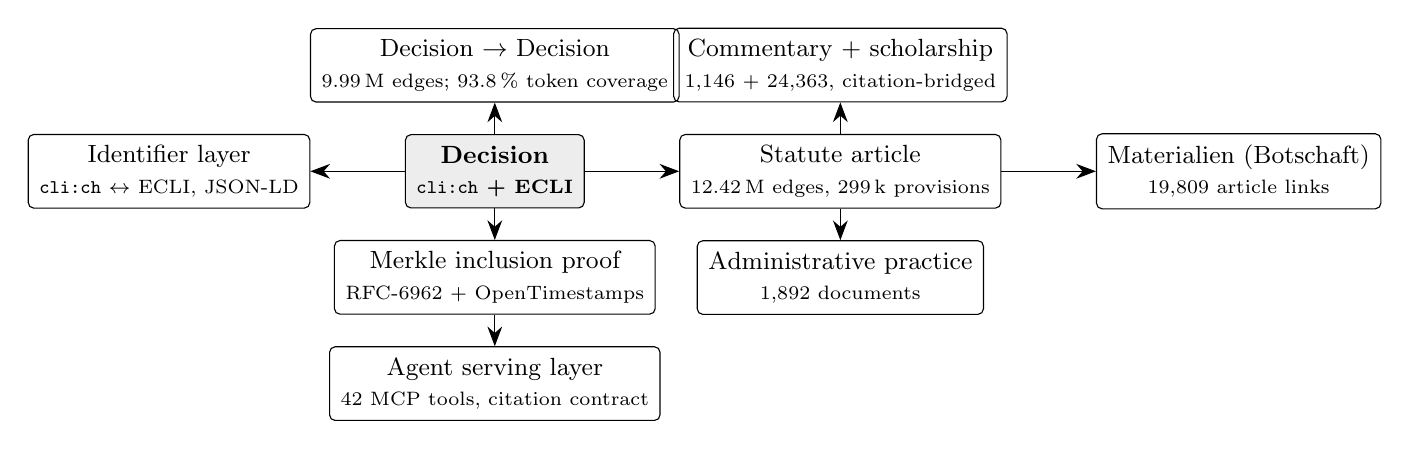
\begin{tikzpicture}[
  node distance=4mm and 12mm,
  every node/.style={font=\small},
  box/.style={draw, rounded corners=2pt, minimum height=8mm, minimum width=22mm, inner sep=4pt, align=center},
  decision/.style={box, fill=black!7, font=\small\bfseries},
  layer/.style={box},
  >={Stealth[length=2.5mm]},
]
\node[decision] (d) {Decision\\\scriptsize \texttt{cli:ch} + ECLI};
\node[layer, above=of d] (c) {Decision $\to$ Decision\\\scriptsize 9.99\,M edges; 93.8\,\% token coverage};
\node[layer, right=of d] (s) {Statute article\\\scriptsize 12.42\,M edges, 299\,k provisions};
\node[layer, below=of d] (i) {Merkle inclusion proof\\\scriptsize RFC-6962 + OpenTimestamps};
\node[layer, left=of d] (k) {Identifier layer\\\scriptsize \texttt{cli:ch} $\leftrightarrow$ ECLI, JSON-LD};
\node[layer, above=of s] (kk) {Commentary + scholarship\\\scriptsize 1{,}146 + 24{,}363, citation-bridged};
\node[layer, right=of s] (m) {Materialien (Botschaft)\\\scriptsize 19{,}809 article links};
\node[layer, below=of s] (pr) {Administrative practice\\\scriptsize 1{,}892 documents};
\node[layer, below=of i] (mcp) {Agent serving layer\\\scriptsize 42 MCP tools, citation contract};
\draw[->] (d) -- (c);
\draw[->] (d) -- (s);
\draw[->] (d) -- (i);
\draw[->] (d) -- (k);
\draw[->] (s) -- (kk);
\draw[->] (s) -- (m);
\draw[->] (s) -- (pr);
\draw[->] (i) -- (mcp);
\end{tikzpicture}%
}
\caption{Resource shape. Decisions form the hub of seven resource layers: case-to-case citations (9.99\,M edges); decision-to-statute references (12.42\,M edges); statute-article anchors to legislative-history Materialien (19{,}809 links), scholarly commentaries and open-access scholarship (1{,}146 + 24{,}363, with a bidirectional decision/statute citation bridge), and federal administrative practice (1{,}892 documents); a layered identifier (\texttt{cli:ch} + ECLI); per-decision cryptographic inclusion proofs (RFC-6962 + OpenTimestamps); and a deployed agent-consumable serving layer under a citation-integrity contract. Individual records need not have an edge to every surrounding layer.}
\label{fig:schema}
\end{figure}

%==================================================================
\section{Related work}\label{sec:related}

\paragraph{Open legal corpora and citation graphs (international).} The Caselaw Access Project~\cite{cap2018} releases 6.7\,M US decisions; Harvard's Library Innovation Lab released a CAP citation graph as a static CSV in 2020.\footnote{Library Innovation Lab, \emph{Caselaw Access Project Citation Graph}, 2020-04-22, \url{https://lil.law.harvard.edu/blog/2020/04/22/caselaw-access-project-citation-graph/}.} CAP is a single-country, predominantly English corpus; its published graph is not paired with a statute graph or legislative-history bridge --- but it demonstrates the substrate-to-benchmark pipeline we aim to enable: CLERC~\citep{hou2024clerc} builds a large-scale case-retrieval and retrieval-augmented-generation benchmark directly on CAP. The \emph{Open Legal Data} platform~\cite{ostendorff2020} releases German court decisions with a citation network covering law and court nodes; follow-up work uses those graphs for joint citation prediction over heterogeneous legal networks~\citep{milz2025missinglink}. \emph{LeCNet}~\cite{lecnet2025} introduces an Indian citation-network benchmark (26\,k nodes); a 2026 Ukrainian release extracts 502\,M citation links from 99.5\,M decisions over a national monolingual corpus~\citep{ovcharov2026ukraine}. \citet{floro2026} benchmark implicit-citation detection in French decisions, illustrating that citation extraction is contested ground even within one jurisdiction. \emph{Pile of Law}~\cite{pile2022} and \emph{MultiLegalPile}~\cite{niklaus2023} are pretraining corpora and do not publish a resolved citation graph at this scale.

\paragraph{Legal-RAG benchmarks need substrates.} LegalBench-RAG~\citep{pipitone2024} and reasoning-focused retrieval benchmarks~\citep{zheng2025} evaluate the retrieval step of legal RAG; claim-level benchmarks extend this to fine-grained attribution~\citep{xu2026claim}. All presuppose a retrieval substrate with stable identifiers and checkable citations --- for US law typically CAP or proprietary corpora. For Swiss law no comparable graph substrate existed; this release is positioned one layer below such benchmarks, as infrastructure on which they can be built (the companion paper contributes retrieval diagnostics).

\paragraph{Swiss legal NLP benchmarks and datasets.} Five task benchmarks on Swiss legal text precede our resource: \emph{Swiss-Judgment-Prediction}~\cite{niklaus2021}; the \emph{One Law, Many Languages} benchmark~\cite{stern2024}; \emph{Criticality Prediction}~\citep{stern2025criticality}; \emph{Swiss Landmark Decisions Summarisation}~\cite{rolshoven2025}; and \emph{SwiLTra-Bench}~\cite{niklaus2025swiltra}. The Swiss Federal Supreme Court Dataset (SCD) records 120{,}368 Federal Supreme Court cases through 2023 with structured metadata~\citep{geering2024scd}. These resources target specific downstream tasks or one federal-court layer; they do not publish a resolved cross-court citation graph, a statute-anchored Materialien layer, or a deployed retrieval endpoint. The Federal Supreme Court layer they represent is one of 28 jurisdictional layers we federate; \citet{stern2025criticality} uses BGE citation patterns as label signal but does not release the underlying cross-court graph.

\paragraph{Agent-accessible legal infrastructure.} The Model Context Protocol~\citep{mcpsurvey2025} is a widely used integration protocol between LLM agents and external tools. Section~\ref{sec:serving} describes the MCP interface and reports operator-side adoption telemetry with explicit measurement caveats.

\paragraph{Comparison.} Table~\ref{tab:comparison} positions OpenCaseLaw against prior releases. Inclusion criterion: open releases that publish a retrieval substrate over court-decision text (a citation graph, a statute-decision link layer, or a live retrieval endpoint) against which downstream RAG and legal-research pipelines can be built. Excluded: task benchmarks and pretraining corpora, discussed above. SCD is a borderline case (structured metadata over BGer, no graph layer); we include it to make the criterion transparent.

\begin{table}[H]
\centering
\caption{Comparison of selected open legal-data resources along dimensions relevant for retrieval-augmented legal research. ``Citation graph'' = resolved citation network; ``Statute graph'' = decision-to-statute-article edges with resolved targets; ``Interp.\ bridges'' = links from provisions/decisions to interpretive sources (legislative history, commentary, scholarship, administrative practice) at document or article granularity; ``Live API'' = continuously served retrieval endpoint (MCP and/or REST). ``Cross-lang links'' = the resource publishes a link layer where edges span $\geq$2 official languages.}
\label{tab:comparison}
\small
\resizebox{\textwidth}{!}{%
\begin{tabular}{l l c l l l c}
\toprule
Resource & Jurisdiction & Cross-lang links & Citation graph & Statute graph & Interp.\ bridges & Live API \\
\midrule
Caselaw Access Project~\cite{cap2018} & US      & no  & static CSV & no  & no  & no  \\
Open Legal Data~\cite{ostendorff2020} & Germany & no  & law/court nodes & no article graph & no  & yes (REST) \\
LeCNet~\cite{lecnet2025}              & India   & no  & 26k bench  & no  & no  & no  \\
Ukrainian citation graph~\citep{ovcharov2026ukraine} & Ukraine & no & 502M extracted links & no & no & no \\
SCD~\citep{geering2024scd}            & CH      & no  & metadata variables & no & no & no \\
\emph{OpenCaseLaw}                    & CH (+ECtHR) & yes & yes, 9.06M resolved & yes, 12.42M edges & yes, 4 layers & yes (MCP+REST) \\
\bottomrule
\end{tabular}%
}
\end{table}

%==================================================================
\section{Corpus}\label{sec:corpus}

The OpenCaseLaw corpus comprises \textbf{1{,}050{,}981 decisions} from \textbf{118 distinct courts} across \textbf{26 Swiss cantons plus federal and ECtHR jurisdictions} (28 jurisdictional layers). Coverage spans \textbf{1875--2026} and three official languages: German (500{,}183 / 47.6\,\%), French (460{,}009 / 43.8\,\%), Italian (90{,}789 / 8.6\,\%). The federal Supreme Court (BGer) is refreshed hourly (Mon--Fri 05:00--16:00 UTC) via a dedicated Neuheiten poller; the remaining collections are refreshed by a nightly publish. The federation aggregates source-specific scrapers and adapters covering federal courts (BGer, BGE, BVGer, BStGer, BPatGer), per-canton portals, the European Court of Human Rights, historical archives, and federal regulatory authorities (FINMA, WEKO, and five others). A snapshot-day check found all 40 decisions published by the Federal Supreme Court on 2026-07-30 serving by mid-morning of the same day.

\paragraph{ECtHR layer.} European Court of Human Rights jurisprudence (\textbf{2{,}879 decisions}: 1{,}199 chamber + 101 grand-chamber + 245 committee + 847 HUDOC entries + 487 BGE-EGMR mirror) is integrated as a first-class federation, refreshed daily against HUDOC. The Court publishes authoritative texts in English and French; the current HUDOC ingestion selects the French authoritative version. Cross-jurisdiction retrieval nevertheless remains multilingual because the Swiss corpus is in German, French, and Italian. ECtHR-origin texts carry distinct licensing (\copyright~ECHR-CEDH; Section~\ref{sec:datacard}).

\paragraph{Completeness.} Some source portals impose access restrictions (geographic, rate, or contractual). We document affected sources in the per-source coverage report, do not claim full coverage where access is restricted, and use only legally authorised collection methods. For closed historical archives where contemporaneous collection is no longer possible, we recover from publicly archived snapshots (e.g.\ Wayback Machine; $\sim$903 BL ALS judgments). The public issue workflow makes coverage defects operationally correctable: between 2026-07-26 and 2026-07-29, five externally filed issue reports (silent truncation, pool-derived result totals, chamber misattribution, identifier encoding, query-syntax handling) were each reproduced, fixed, and converted into permanent regression tests; the chamber report alone corrected $\sim$54{,}000 stored rows (Section~\ref{sec:infra}).

\paragraph{Licensing.} Court decisions in Switzerland are official acts under URG/CopA Art.~5 (excluded from copyright). Corpus packaging is CC0; code is MIT; commentaries retain their upstream CC-BY-4.0 / CC-BY-SA-4.0 terms; ECtHR-origin texts are \copyright~ECHR-CEDH and are served with attribution and excluded from the CC0 Parquet export (Section~\ref{sec:datacard}).

%==================================================================
\section{Multilingual citation graph}\label{sec:graph}

\paragraph{Denominator taxonomy.} Counts in this section use one frozen 2026-07-30 snapshot. We use four distinct denominators:
\begin{itemize}\setlength{\itemsep}{2pt}\setlength{\parskip}{0pt}
\item $E_{\textrm{extracted}} = \textbf{9{,}663{,}853}$: distinct (source-decision, citation-token) pairs extracted by full-text scan over the corpus.
\item $E_{\textrm{resolved}} = \textbf{9{,}061{,}243}$: subset of $E_{\textrm{extracted}}$ whose token resolves to $\geq 1$ target decision (93.8\,\%).
\item $E_{\textrm{link}} = \textbf{9{,}989{,}926}$: rows of the published \texttt{citation\_targets} table, expanded for target multiplicity (a small fraction of citation tokens resolve to multiple targets, e.g.\ BGE form references that match several published BGEs by docket, and decisions stored under both a legacy and a canonical identifier).
\item $E_{\textrm{link,lang}} = \textbf{9{,}989{,}926}$: subset of $E_{\textrm{link}}$ where both source and target language are in $\{$de, fr, it$\}$; in this snapshot, all link rows satisfy this.
\end{itemize}
The cross-lingual share (34.2\,\%, Section~\ref{sec:intro}) is computed over $E_{\textrm{link,lang}}$; the 93.8\,\% resolution rate is computed over $E_{\textrm{extracted}}$. The precision proxies below are computed over $E_{\textrm{link}}$ on the same frozen graph, grouped by \texttt{match\_type}.

\begin{table}[H]
\centering
\caption{Citation graph. Edges extracted by full-text scanning every decision in the corpus; resolved means the cited target is identified in the corpus. Snapshot 2026-07-30.}
\label{tab:citation_graph}
\small
\begin{tabular}{l r}
\toprule
\textbf{Quantity} & \textbf{Value} \\
\midrule
Decisions analysed for outgoing citations & 1,050,979 \\
Citation edges (source $\to$ target reference) & 9,663,853 \\
Edges with target resolved to a corpus decision & 9,061,243 (93.8\%) \\
Distinct decisions cited at least once & 311,166 \\
Decisions cited $\geq$ 100 times & 13,682 \\
Decisions cited $\geq$ 1{,}000 times & 1,245 \\
Decisions cited $\geq$ 10{,}000 times & 55 \\
\bottomrule
\end{tabular}
\end{table}

\begin{table}[H]
\centering
\caption{Cross-lingual citation matrix. Rows are source decision languages; columns are cited (target) decision languages. Cells give resolved citation edges. Off-diagonal = 3,416,520 / 9,989,926 = 34.2\% of resolved citations with identified source and target language.}
\label{tab:cross_lang_citation}
\small
\begin{tabular}{l r r r}
\toprule
& \textbf{$\to$ DE} & \textbf{$\to$ FR} & \textbf{$\to$ IT} \\
\midrule
\textbf{DE $\to$} & 3,848,162 & 627,011 & 50,306 \\
\textbf{FR $\to$} & 2,049,708 & 2,621,336 & 66,157 \\
\textbf{IT $\to$} & 434,638 & 188,700 & 103,908 \\
\bottomrule
\end{tabular}
\end{table}

\FloatBarrier

\paragraph{Resolution at scale.} We extract citation tokens by full-text scanning every decision in the corpus (\textbf{1{,}050{,}979} decisions in the reference-graph snapshot; the FTS5 search index carries 2 more, ingested between graph rebuild and index swap), recovering $E_{\textrm{extracted}} = \textbf{9{,}663{,}853}$. Resolution runs three exact-match passes (general docket-normalisation; BGE/ATF/DTF prefix-form; bare BGE numeric form), then a \emph{pin-cite-aware fallback} for Swiss legal citations such as \emph{BGE 125 V 352} that pinpoint into the body of a case starting at \emph{BGE 125 V 351} (the pin-cite resolver matches each unresolved BGE-form reference to the nearest preceding first-page in the same volume\,$+$\,division within 30 pages, contributing \textbf{934{,}734} link rows at a $-$0.10 confidence discount), and finally an \emph{additive cross-reference stratum} (\texttt{oracle\_xref}, \textbf{29{,}856} link rows) that recovers citations naming a BGer docket whose decision is stored under its BGE publication number, via the docket$\leftrightarrow$BGE cross-reference extracted from BGE headers. Each stratum is insert-only over the previous ones, so improvements are additive and auditable per \texttt{match\_type}. The 93.8\,\% rate is a 0.9\,pp lift over the 2026-05-21 release (92.9\,\%) and an 18.6\,pp lift over the internal pre-fix baseline of 75.2\,\%.

\paragraph{Heavy-tailed centrality.} The citation graph is heavy-tailed (Table~\ref{tab:citation_graph}): 55 decision identifiers are cited 10{,}000+ times, 1{,}190 are cited 1{,}000--9{,}999 times, and most cited decisions sit in the long tail. The single most-cited decision is BGE 125 V 351 (the leading case on evidentiary standards in social-insurance law), with \textbf{100{,}760} distinct citing (source, token) pairs after aggregating its two stored identifier variants. Of the 50 most-cited decisions, the large majority are DE-originals --- a distinct cut of the graph (citation reception, not direction).

\paragraph{Precision proxies.} The 93.8\,\% resolution number is a \emph{coverage} metric and does not bound precision. To characterise precision risk we compute automated proxies (Table~\ref{tab:precision_proxies}). The proxies surface \emph{recorded-date chronology violations}: each detected case is a logical inconsistency \emph{conditional on the source and target decision dates being themselves correct}. We preserve source-portal-provided dates (Section~\ref{sec:limit}), so a violation is a strong but not infallible indicator of a false-positive resolution; date-consistent pairs may still be false positives for reasons the proxies do not see. \emph{Date-order sanity} (target decision not dated after source) finds violations in \textbf{2.04\,\%} of $E_{\textrm{link}}$ rows with both dates known. This places the date-sanity-visible precision ceiling at \textbf{97.96\,\%} on date-covered pairs conditional on the recorded dates; it does \emph{not} establish a lower bound on precision. Per-stratum, the exact-match BGE strata sit lowest (bge\_bare 0.61\,\%, bge\_norm 1.02\,\%), the pin-cite heuristic's violation rate fell to 2.01\,\% (2.65\,\% in the 2026-05 release), the high-volume docket stratum sits at 2.70\,\%, and the new \texttt{oracle\_xref} stratum is the noisiest at 6.51\,\% --- small in volume (30\,k rows) but flagged accordingly; its rows carry a reduced confidence score. The weighted rate rose from 1.53\,\% to 2.04\,\% between releases, driven by docket-stratum growth --- movement we report rather than smooth over. \emph{Self-citation} is zero across all link rows.

\begin{table}[t]
\centering
\caption{Citation-resolution precision proxies from a quality-control run over 8,097,538 resolved pairs. Date-sanity pass = \% of pairs where target decision date is not after the source's; violations are logical impossibilities and thus a hard floor on false-positive count, not a lower bound on precision. Self-cite = pairs where source = target. Conf.\,p50 = median resolver confidence per stratum. Full per-stratum manual precision adjudication is deferred to v2.0 (see \texttt{benchmarks/citation\_precision\_audit.py}).}
\label{tab:precision_proxies}
\small
\begin{tabular}{l r r r r}
\toprule
\textbf{match\_type} & \textbf{n} & \textbf{date sanity} & \textbf{self-cite} & \textbf{conf p50} \\
\midrule
\texttt{docket\_norm} & 3,286,234 & 97.25\% & 0 & 0.99 \\
\texttt{bge\_bare} & 2,943,028 & 99.75\% & 0 & 0.85 \\
\texttt{bge\_norm} & 1,215,768 & 99.26\% & 0 & 0.75 \\
\texttt{bge\_pincite} & 652,508 & 97.35\% & 0 & 0.75 \\
\midrule
\textbf{Overall} & 8,097,538 & 98.47\% & 0 & --- \\
\bottomrule
\end{tabular}
\end{table}

\FloatBarrier

\paragraph{Rule-based consistency adjudication on the 400-sample audit set.} As an orthogonal complement to the chronology proxy, we ship a mechanical per-row consistency adjudication over a 400-row stratified audit set (\path{benchmarks/citation_precision_sample_400.jsonl}; rules at \path{benchmarks/citation_precision_audit_rules.py}), drawn from and frozen with the 2026-05-21 release. Each row is checked against the documented per-stratum canonicalisation rules: BGE-form parsing for \texttt{bge\_bare}/\texttt{bge\_norm}; docket-pattern suffix matching for \texttt{docket\_norm}; the 30-page window for the pin-cite heuristic. Result: \textbf{400/400 samples} pass (Wilson 95\,\% CI [99.0\,\%, 100.0\,\%] for the checked property; bge\_bare 100/100, bge\_norm 80/80, bge\_pincite 100/100, docket\_norm 120/120). This is evidence that the published target identifiers are mechanically consistent with the resolver's own rules on this sample. It does \emph{not} verify semantic correctness: whether the resolver picked the right case when multiple cases share a docket pattern, whether a rule-consistent pin-cite points into the intended case, or whether the source text correctly identified the cited decision remains companion-paper scope (multi-annotator human adjudication). The audit set predates the \texttt{oracle\_xref} stratum, which is therefore not represented in it.

\paragraph{Cross-language citation flow.} Table~\ref{tab:cross_lang_citation} shows the language-by-language citation matrix over $E_{\textrm{link,lang}} = 9{,}989{,}926$, as a descriptive cut of the released graph. The aggregate cross-language share is \textbf{34.2\,\%}. Row-normalisation by source language exposes the asymmetry: German-language decisions cite outside German in only \textbf{15.0\,\%} of resolved links; French in \textbf{44.7\,\%}; Italian in \textbf{85.7\,\%}. FR$\to$DE links (\textbf{2.05\,M}) outweigh DE$\to$FR (\textbf{0.63\,M}) by \textbf{3.3$\times$}. The ratios cover the full population of language-known link edges, so there is no sampling uncertainty, but there is measurement uncertainty from unresolved tokens and possible language-pair resolution bias. We make no structural-cause claim from this matrix alone (Section~\ref{sec:limit}).

%==================================================================
\section{Statute graph and interpretive bridges}\label{sec:statutes}

Swiss statutory interpretation is methodologically plural: courts consider a provision's text, context, purpose, legislative history (\emph{Materialien}), and other interpretive sources. The substrate makes several such layers programmatically reachable from the provision.

\paragraph{Statute graph.} We resolve \textbf{12{,}423{,}168 decision-to-statute edges} touching \textbf{298{,}922 distinct provisions}. The statute layer is grounded in two parallel mirrors: a federal layer of \textbf{5{,}525 SR-numbered Fedlex laws} (401{,}313 article rows summed across the parallel DE/FR/IT versions) and a cantonal layer of \textbf{15{,}600 laws} (361{,}568 articles) covering all 26 cantons via direct portal scraping (LexWork, 18 cantons; SIL, 2; ZH OpenData; TI RL), with LexFind PDF fallback supplementing cantons whose primary portals miss laws. The cantonal law count is $\sim$120 lower than the 2026-05 release after cross-portal deduplication --- corpus counts can legitimately move in both directions as quality passes land. Alias canonicalisation across major DE/FR/IT statute abbreviations is lexical only; temporal validity (mapping a 1998 \emph{OG} reference to its current SR location, or distinguishing repealed-vs-current article versions) is left for future work.

\begin{table}[H]
\centering
\caption{Statute and doctrinal graph layers. Decision-to-statute edges plus federal/cantonal mirrors plus Materialien (Federal Council Botschaften) and open commentaries.}
\label{tab:statute_graph}
\small
\begin{tabular}{l r}
\toprule
\textbf{Quantity} & \textbf{Value} \\
\midrule
Decision $\to$ statute edges & 12,423,168 \\
Distinct provisions referenced & 298,922 \\
\addlinespace
Federal laws (Fedlex SR series) & 5,525 \\
Federal articles (DE/FR/IT parallel) & 401,313 \\
Cantonal laws (all 26 cantons; 22 direct, 4 LexFind fallback) & 15,600 \\
Cantonal articles & 361,568 \\
\addlinespace
Materialien (Botschaft documents, DE/FR/IT) & 6,154 \\
Materialien paragraphs (full-text) & 421,489 \\
Article-anchored Materialien links & 19,809 \\
\addlinespace
Open commentaries (CC-BY/CC-BY-SA) & 1,146 \\
\bottomrule
\end{tabular}
\end{table}

\FloatBarrier

\paragraph{Materialien bridge.} A distinguishing feature of Swiss civil-law interpretation is the \emph{teleological} reading of statutes via \emph{Materialien}. We discover Botschaft documents via the Fedlex JOLUX SPARQL endpoint and parse \textbf{6{,}154} documents (\textbf{421{,}489} full-text paragraphs) from Akoma Ntoso XML where available, PDF fallback otherwise. Anchoring traverses the official parliament chain (\texttt{parliamentDraftId} $\to$ enacted \texttt{oc} $\to$ codified \texttt{cc} $\to$ \texttt{SR}), yielding \textbf{19{,}809} article-to-Botschaft links covering \textbf{620 statutes} and \textbf{12{,}232 distinct articles} --- a 2.4$\times$ expansion over the 2026-05 release. The links derive from the statutes' own AS/BBl amendment footnotes, so their relation is ``this message concerns that article'', never ``this is the enacting message''; retrieval interfaces state this. A small curated digest layer (167 article-level intent summaries for two anchor laws) sits on top; the serving layer discloses on every response which of the two layers answered, after an audit found that an empty digest read as ``Switzerland has no preparatory materials'' --- false for a shelf holding 6{,}154 messages. Known failure modes of the anchoring (rejected drafts lacking an enacted side; multi-statute omnibus messages inflating link counts; post-renumbering anchors) are documented with the layer; we have not yet computed an end-to-end precision audit for the anchoring, so this release treats it as a high-recall legislative-history discovery index rather than an adjudicated alignment benchmark.

\paragraph{Commentaries and open-access scholarship.} We bridge \textbf{1{,}146} scholarly commentaries (CC-BY-4.0 from OnlineKommentar.ch; CC-BY-SA-4.0 from OpenLegalCommentary.ch) into the graph, anchored by SR number plus article --- a 3.2$\times$ growth over the 2026-05 release under the upstream projects' own publication cadence. A new scholarship layer federates \textbf{24{,}363} open-access publications from \textbf{23 Swiss repositories} (university archives, OA journals, institutional collections), with per-record licence retention and a \emph{bidirectional citation bridge}: publications are linked to the decisions and statute articles they cite (19{,}044 publication$\to$decision and 37{,}713 publication$\to$statute-article edges), so a decision's page can list the literature discussing it, and a provision's page the scholarship interpreting it. Full text is retrieved where the upstream licence permits; otherwise metadata and links only.

\paragraph{Administrative practice.} Federal agencies operationalise statutes through circulars, guidance and article-by-article commentary that courts routinely engage with. The practice layer ships \textbf{1{,}892} documents: SECO's article-by-article commentary on the employment act and its five ordinances (1{,}102 documents, DE/FR/IT), ESTV tax circulars and VAT guidance (438), BAFU environmental implementation aids (297), and SEM migration directives (55); DE 866 / FR 514 / IT 512. Each document carries issuing authority, document number, date, language and source PDF; the corpus is FTS-indexed and statute-anchored where the source is article-keyed (SECO). Coverage is partial by construction --- several major authorities (BSV, FINMA, BAG, cantonal administrations) are not yet ingested and the serving layer says so in-band rather than letting an empty result imply the practice does not exist.

%==================================================================
\section{Identifier and provenance layer}\label{sec:provenance}

\paragraph{Layered identifier (cli:ch + ECLI).} Every decision carries a Swiss-native canonical identifier \texttt{cli:ch} with a Council-of-EU ECLI projection, both surfaced in the per-decision Schema.org/LegalCase JSON-LD. cli:ch makes three features first-class that an ECLI-only scheme flattens: (i)~\emph{trilingualism} (DE/FR/IT versions of a BGE are legally equally authentic per Art.~14 PublG; cli:ch treats language as a first-class axis via \texttt{?lang=}); (ii)~\emph{cantonal + chamber granularity} (\texttt{cli:ch:zh:obergericht:...} preserves the 26 cantonal systems and their chambers rather than collapsing to an opaque court code); (iii)~\emph{pinpoint addressing} (Erwägung-level fragments like \texttt{\#e-2.3}, matching the Schweizer-Citation convention). An optional \texttt{@YYYY-MM-DD} suffix addresses a specific anonymisation version when needed. The compact form is
\begin{center}
\texttt{cli:ch:<court>[:<chamber>]:<docket>[@<version>][?lang=<l>][\#<pinpoint>]}.
\end{center}
The mapping to ECLI is a pure function (\texttt{cli\_ch\_to\_ecli}); the projection is many-to-one (lossy on language, pinpoint, version, chamber detail). An HTTP resolver at \url{https://opencaselaw.ch/cli/ch/} plus the court/chamber/docket path redirects to the canonical decision page; browsers preserve fragment pinpoints across the 302. Identifier hygiene is enforced at the serving layer: legacy identifier forms containing spaces ($\sim$5.6\,\% of stored ids) are percent-encoded at every URL construction site, with a source-scan regression test pinning the invariant after an external report showed truncated links producing non-unique identifiers.

\paragraph{Cryptographic provenance (RFC-6962 + OpenTimestamps).} Every daily publish computes an RFC-6962 Merkle tree over all decisions in the corpus. Each leaf commits to the tuple \texttt{(decision\_id, cli:ch, ECLI, content\_hash, decision\_date)}. We commit the 32-byte SHA-256 root (hash-domain-separated per the Certificate-Transparency RFC) to the public Git repository at \path{docs/integrity/<YYYY-MM-DD>.root} and anchor it on the Bitcoin blockchain via OpenTimestamps (\path{.root.ots}). The root for the present snapshot, over 1{,}050{,}981 decisions on 2026-07-30, begins \texttt{f5fc6229}. A \texttt{GET /api/integrity/<decision\_id>} endpoint returns an inclusion proof in $O(\log n) \approx 20$ sibling hashes, computed in milliseconds against a memoised subtree cache. Any client can independently verify that a given decision was in the corpus on a given date without trusting the server: leaf $\to$ inclusion-proof walk $\to$ root $\to$ OpenTimestamps proof $\to$ Bitcoin block. Inclusion verification thus becomes a public API surface, not an internal release-engineering detail.

\paragraph{Standards proposal.} Six elements appear together as an open-standards proposal at the \emph{Standards} URL in Section~\ref{sec:open}: the identifier convention; the JSON-LD metadata schema; Akoma Ntoso for legislative materials; Markdown with pinpoint anchors for full text; the resolved-citation conventions used here; and the Merkle-plus-OpenTimestamps provenance layer. Each is independently adoptable.

%==================================================================
\section{Agent-native serving layer and measured adoption}\label{sec:serving}

Legal-research consumers include LLM agents, and a static dump alone does not expose serving-time constraints or coverage notices. OpenCaseLaw is therefore served natively over the Model Context Protocol~\citep{mcpsurvey2025}: \textbf{42 public MCP tools} (search across every layer; per-Erwägung pinpoint retrieval; citation-graph walks; statute, Materialien, commentary, scholarship and practice lookups; batch retrieval; a deep-research shim) alongside REST with an OpenAPI subset and a daily CC0 Parquet export.

\paragraph{A citation-integrity serving contract.} The tool contract encodes practices motivated by the hallucination literature~\cite{dahl2024,magesh2024,charlotin2026}: (i)~every citation string returned by a tool is copied from the stored record, never constructed --- tools expose \texttt{citation\_string\_de/fr/it} fields and a \texttt{cite} tool, and the server instructs clients not to assemble citations; (ii)~verbatim quotation is available through tools that return stored text spans (per-Erwägung, per-regeste, per-article), giving a quoting client a provenance chain to the source; (iii)~honest emptiness --- tools disclose coverage limits in-band (``no digest exists for this law; the linked messages are\dots'') rather than returning silent zeros, after audits showed empty results being read as substantive legal facts; (iv)~machine-readable disclosure of truncation and lower-bound result totals. We regard these as serving-layer obligations of a legal resource, on par with licensing: the interface can expose the substrate's evidentiary constraints to its consumers.

\paragraph{Measured adoption.} Because the endpoint is operated infrastructure, usage is observable operator-side. Over the 30 days to 2026-07-30 (Table~\ref{tab:adoption}): $\sim$15.1\,M API calls and $\sim$1.54\,M MCP transport opens or requests; AI-assistant clients on three platforms sustained daily use (Claude-family clients $\sim$16--23\,k tool calls/day; ChatGPT-family clients episodic with a three-week high-volume campaign; Microsoft-Copilot integrations at two law firms). The traffic also included a self-identifying corpus harvester (User-Agent naming its operator and purpose) and a templated monitor issuing $\sim$45\,k standardised social-insurance queries per day within two days of its first appearance, patterns consistent with programmatic or autonomous operation. Roughly 79\,\% of raw call volume is bulk corpus export by a handful of programmatic consumers; the interactive research layer beneath it is the smaller but analytically distinct signal. Web readership of decision pages runs at $\sim$2{,}500--3{,}500 distinct visitors per day, almost entirely search-engine-referred single-case reads.

\begin{table}[H]
\centering
\caption{Operator-side adoption telemetry, 30 days to 2026-07-30. Client families are classified from request metadata (User-Agent heuristics). The MCP counter mixes transport opens with requests and is not a count of people or deduplicated protocol sessions. Web-visitor counts are distinct daily IP addresses on decision pages after removing bot and datacentre traffic, with residential-proxy inflation filtered by page/asset behaviour. Classification error can move class-specific and visitor counts in either direction; counter resets or missed terminal flushes bias reconstructed API totals downward.}
\label{tab:adoption}
\small
\begin{tabular}{L{0.42\textwidth} r}
\toprule
\textbf{Measure (30 days)} & \textbf{Value} \\
\midrule
API calls (all surfaces)            & $\sim$15.1\,M \\
\quad of which bulk corpus export   & $\sim$79\,\% \\
MCP transport opens / requests      & $\sim$1.54\,M \\
Claude-family client calls          & $\sim$0.5\,M \\
ChatGPT-family client calls         & $\sim$0.3\,M \\
Command-line agent (claude-code) calls & $\sim$51\,k \\
Word add-in citation checks         & $\sim$7.4\,k/month \\
Distinct human web visitors / day   & $\sim$2{,}500--3{,}500 \\
\bottomrule
\end{tabular}
\end{table}

We report these figures as \emph{adoption evidence with caveats}, not as an evaluation: client families are User-Agent heuristics; the MCP counter does not identify people or deduplicated sessions; a single consumer can dominate a row; and the reconstruction from cumulative per-worker counters is conservative but not exact. The methodological point is that operating a substrate exposes access patterns that a static release would not reveal directly. These observations motivated serving-layer changes including input-length caps with instructive errors, query condensation for pasted documents, and per-tool functional monitoring.

%==================================================================
\section{Dataset health}\label{sec:infra}

Four layers guard the release (Table~\ref{tab:qa_layers}).

\begin{table}[H]
\centering
\caption{Quality assurance, by layer. L1--L3 are publish-blocking on a critical regression (the orchestrator refuses to advance to the git-push step). L4 is alerting-only.}
\label{tab:qa_layers}
\small
\resizebox{\textwidth}{!}{%
\begin{tabular}{l l l l l}
\toprule
\textbf{Layer} & \textbf{Scope} & \textbf{Granularity} & \textbf{Frequency} & \textbf{Blocks publish?} \\
\midrule
L1 & function tests           & 1{,}568 pytest cases                                       & every CI push     & yes \\
L2 & build-time pipeline      & normalisation + correction passes in \texttt{build\_fts5.py} & nightly rebuild   & yes \\
L3 & dataset audit            & 72 \texttt{check\_*} functions / 22 modules                & nightly rebuild   & yes \\
L4 & production smoke + tool surface & 8 endpoint probes / 5\,min; all-42-tool functional check daily & continuous & alerts only \\
\bottomrule
\end{tabular}%
}
\end{table}

L3 publishes per-check JSON at \url{https://opencaselaw.ch/quality.json}, refreshed every nightly rebuild. Publish-blocking critical conditions: total-count cliff $>$1\,\%, schema break, court not in registry, future-date count $>$50, cross-DB row-count mismatch $>$0.5\,\%. The L4 tool-surface check calls all 42 MCP tools daily with realistic arguments and identifiers harvested from live searches, so a tool that answers with an error, an empty payload, or an unreachable identifier chain alerts the operator the same day --- added after an audit found failure classes (an error string returned as an answer on the zero-result path; a tool whose required input no other tool emitted) that endpoint-level smoke checks do not exercise. We codify production incidents and externally reported issues as permanent regression tests; the 2026-07 cycle converted five external reports into fixes with tests, including a build-time re-derivation that corrected the chamber attribution of $\sim$54{,}000 Federal Supreme Court records.

%==================================================================
\section{Data card}\label{sec:datacard}

\begin{table}[H]
\centering
\caption{Data card. Frozen 2026-07-30 release; live state always at \url{https://opencaselaw.ch}.}
\label{tab:datacard}
\small
\begin{tabular}{L{0.24\textwidth} L{0.69\textwidth}}
\toprule
\textbf{Field} & \textbf{Value} \\
\midrule
Sources              & Federal courts (BGer, BGE, BVGer, BStGer, BPatGer); 26 cantonal portals; ECtHR (HUDOC); federal regulatory authorities (FINMA, WEKO, ED\"OB, UBI, ELCom, PostCom, ComCom); federal agencies (SECO, ESTV, SEM, BAFU) for administrative practice; 23 OA repositories for scholarship; Wayback for closed historical archives \\
Languages            & DE 47.6\,\%, FR 43.8\,\%, IT 8.6\,\% (official versions only; no machine translation) \\
Coverage gaps        & Access-restricted portals documented in per-source coverage report; administrative-practice and scholarship layers partial by construction and disclosed in-band \\
Refresh              & BGer hourly (Mon--Fri 05:00--16:00 UTC); ECtHR daily; all other federations nightly \\
Personal-data posture & FADP; inherit upstream pseudonymisation; no re-pseudonymisation, no de-pseudonymisation; published telemetry is aggregated by actor class; operational request metadata and truncated search traces are retained under documented time limits (search traces auto-deleted after 30 days) \\
Known noise classes  & Encoding drift, HTML-entity contamination, OCR artefacts in historical archives, control-character leakage from PDF extraction, near-duplicate cross-portal content, legacy identifier-form duality (Section~\ref{sec:limit}) \\
Licensing            & Corpus packaging CC0; decision texts under URG/CopA Art.~5 official-acts exclusion; \textbf{ECtHR-origin texts \copyright~ECHR-CEDH}, redistributed under the Court's reuse terms with attribution served alongside the text and \textbf{excluded from the CC0 Hugging Face export} (deny-listed at export time); commentaries CC-BY-4.0 / CC-BY-SA-4.0; scholarship per-record upstream licences; code MIT \\
Removal / correction & \href{https://github.com/jonashertner/caselaw-repo-1/blob/main/docs/governance-and-removal-policy.md}{Public governance-and-removal policy}; verified requests honoured per documented procedure \\
\bottomrule
\end{tabular}
\end{table}

%==================================================================
\section{Limitations}\label{sec:limit}

\paragraph{Citation precision is bounded, not measured.} The 93.8\,\% resolution rate is a coverage metric, not a precision bound. The date-sanity proxy gives a ceiling for date-sanity-visible precision on date-covered pairs, conditional on the recorded source and target dates being correct themselves. The rule-based consistency adjudication finds no rule-visible malformed identifiers or pin-cite range overflows in the 400-sample audit set, which is frozen from the 2026-05-21 release and does not cover the newer \texttt{oracle\_xref} stratum. Neither establishes a \emph{lower} bound on precision. Multi-annotator human adjudication is companion-paper scope.

\paragraph{Identifier-form duality.} $\sim$5.6\,\% of stored decision identifiers exist in a legacy form containing spaces, and some decisions are stored under both a legacy and a canonical identifier; the most-cited decision is itself split across two identifier variants, which the headline centrality numbers aggregate explicitly. URL construction percent-encodes all identifier forms (with a regression test), but identifier normalisation across the corpus --- a migration with citation-graph implications --- is deliberately deferred and documented rather than partially applied.

\paragraph{Temporal validity, source pseudonymisation, snapshot-date semantics.} (i) The statute graph maps references to the \emph{current} SR location; a 1998 \emph{OG} reference resolves to surviving content without distinguishing the original from the superseded version. Versioned statute resolution remains future work. (ii) Source pseudonymisation is inherited. Federal decisions typically arrive pre-pseudonymised; some cantonal decisions arrive unredacted. We neither re-pseudonymise nor de-pseudonymise; removal requests follow the documented governance policy. (iii) Some source portals expose near-future publication dates (the snapshot's maximum recorded decision date is 2026-09-14). We preserve source-provided dates rather than rewriting them, and the dataset-health gate treats large future-date spikes as critical scraper regressions.

\paragraph{Per-language resolution-rate confounder for the cross-language matrix.} The 34.2\,\% aggregate is computed over the released resolved graph. If resolution rates differ systematically by language pair (and the pin-cite-aware resolver was tuned on BGE-form citations, disproportionately DE-original), the share could be biased. Conditional on such bias, our hypothesised direction is attenuation of same-language diagonals and amplification of cross-DE flows; the 34.2\,\% would then be an upper bound rather than an underestimate. Magnitude and direction await the language-pair precision audit (companion paper).

\paragraph{Interpretive bridges are recall-oriented and uneven.} The Materialien anchoring has no end-to-end precision audit and its links mean ``concerns'', not ``enacts''. The scholarship bridge inherits upstream metadata quality and OA coverage bias (institutional repositories over commercial journals). The administrative-practice layer covers four federal agencies; most authorities are absent. In each case the serving layer discloses the limitation in-band; the risk that remains is a consumer treating high recall as completeness.

\paragraph{Adoption telemetry is observational.} The usage figures in Section~\ref{sec:serving} are operator-side measurements with heuristic client classification, not an evaluation of usefulness; they can be dominated by single consumers; and they are reconstructed from cumulative per-worker counters (conservative under counter resets). They evidence use and include substantial agent-classified traffic; they do not establish a longitudinal shift or show that the substrate is used \emph{well}.

\paragraph{Source-text fidelity is upstream-bound.} Decision text quality follows the originating portal. Known noise classes: encoding drift, residual HTML-entity contamination, OCR artefacts in historical archives (BGE 1875--1953, Wayback-recovered BL ALS, MKG), control-character leakage from PDF extraction, and near-duplicate cross-portal content. Build-time normalisation passes catch the common cases. The corpus claims fidelity to what each source portal published, with documented normalisation applied, not to a hypothetical canonical text.

\paragraph{Scope.} The cross-language citation-flow matrix is descriptive characterisation of the released graph, not the resource contribution. The cross-lingual retrieval diagnostic, audit-rail framework, and prior-only-vs-RAG-augmented bench are evaluation contributions that depend on this resource and will be reported in the companion paper once their multi-annotator and human-judge-calibration components are complete.

%==================================================================
\section{Discussion}\label{sec:disc}

\paragraph{What the resource enables, and for whom.} The substrate serves four audiences. For \emph{legal-NLP researchers}: every resolved citation has a stable target identifier and every statute reference is article-anchored, so retrievers, generators, and legal-RAG systems can build on a substrate whose records can be checked for membership in a Bitcoin-anchored snapshot --- the role CAP plays for CLERC~\citep{hou2024clerc}, now available for a multilingual civil-law jurisdiction. For \emph{Swiss legal practitioners}: the live endpoint supports decision lookup, Erwägung-level pinpoint citation, and cross-court reference walks with provenance-anchored data, plus the interpretive layers (Materialien, practice, commentary, scholarship) practitioners actually argue with. For \emph{Swiss courts and public bodies}: the same data products they publish flow back as a federated, identifier-stable corpus with inclusion-proof verification, supporting referential integrity across systems and offering a public auditing surface for the official record. For \emph{civic-tech and legal-aid services}: the same live endpoint is free, machine-readable, and stable; self-help tools and legal-aid clinic interfaces can build against a substrate they can cite, audit, and reproduce, without the institutional-subscription barrier.

\begin{table}[H]
\centering
\caption{Concrete tasks supported by the released substrate. The right column gives the minimal object or query against the live MCP/REST endpoint or the static corpus snapshot.}
\label{tab:reuse}
\small
\begin{tabular}{L{0.32\textwidth} L{0.26\textwidth} L{0.34\textwidth}}
\toprule
\textbf{Task} & \textbf{Resource object} & \textbf{Example} \\
\midrule
Find all cases citing a decision           & citation graph (\texttt{citation\_targets}) & incoming refs to BGE 125 V 351 \\
Build legal RAG over decisions + statutes  & decision + statute graph                    & retrieve a decision plus its cited SR articles \\
Trace statutory intent (teleology)         & Materialien bridge                          & SR-article $\to$ Federal Council Botschaft \\
Find doctrine and literature on a provision & commentary + scholarship bridges           & Art.~336 OR $\to$ commentaries, citing OA papers \\
Check how an agency applies a provision    & administrative-practice layer               & ArG article $\to$ SECO commentary (DE/FR/IT) \\
Verify corpus membership on a given date   & integrity API                               & per-decision inclusion proof vs.\ daily Merkle root \\
Normalise Swiss citations across systems   & \texttt{cli:ch} $\leftrightarrow$ ECLI       & stable identifier across DE/FR/IT versions and chambers \\
Serve agents with citation integrity       & MCP tool layer                              & 42 tools; stored citation strings; honest emptiness \\
\bottomrule
\end{tabular}
\end{table}

\paragraph{Open questions.} Four lines of follow-up work motivated by the resource: (i) precision-controlled measurement of the cross-lingual citation share with a multi-annotator stratified audit; (ii) versioned statute resolution so a 1998 \emph{OG} reference resolves to the contemporaneous statute text; (iii) cross-lingual retrieval evaluation with lawyer-authored held-out queries (companion paper); (iv) longitudinal characterisation of agentic consumption, to test whether the substantial agent-classified traffic observed in this window persists or changes over later release cycles.

%==================================================================
\section{Open access and reproducibility}\label{sec:open}

All artefacts are publicly available:
\begin{itemize}
\item Corpus: Hugging Face \url{https://huggingface.co/datasets/voilaj/swiss-caselaw} (CC0; ECtHR-origin texts excluded per Section~\ref{sec:datacard} and served via the API with attribution)
\item Code: \url{https://github.com/jonashertner/caselaw-repo-1} (MIT)
\item Live MCP/REST: \url{https://mcp.opencaselaw.ch} (42 MCP tools; OpenAPI at \path{/api/openapi.copilot.json})
\item Word add-in (lawyer-facing client): \url{https://opencaselaw.ch/word}
\item Dashboards: \url{https://opencaselaw.ch}, \url{https://opencaselaw.ch/quality.html}
\item Standards proposal: \url{https://opencaselaw.ch/standards/}
\item Integrity / Merkle root and OpenTimestamps anchor: \url{https://opencaselaw.ch/integrity/}
\end{itemize}

\paragraph{Utility demonstration.} The smallest end-to-end demo against the live endpoint:

\begin{quote}\small
\begin{verbatim}
$ curl https://mcp.opencaselaw.ch/api/decisions/bge_BGE_125_V_351
  -> { decision_id, citation_string_de, citation_string_fr,
       citation_string_it, canonical_url, full_text, ... }

$ curl https://mcp.opencaselaw.ch/api/citations/bge_BGE_125_V_351
  -> { decision_id, direction, incoming: [...], outgoing: [...] }

$ curl https://mcp.opencaselaw.ch/api/integrity/bge_BGE_125_V_351
  -> { decision_id, root_date: "2026-07-30",
       root: "f5fc6229...",
       inclusion_proof: [ ~20 sibling hashes ] }
\end{verbatim}
\end{quote}

\noindent The first call returns the canonical decision record and citation strings; the second exposes its citation-graph neighbourhood; the third returns a cryptographic membership proof that lets any client verify the decision was in the 2026-07-30 release snapshot without trusting the server: traverse the inclusion proof, recover the daily Merkle root, then verify that root against the OpenTimestamps Bitcoin anchor.

\paragraph{Reproducibility capsule.} Corpus and graph counts derive from the frozen snapshot at \path{docs/paper/p1-resource/tables/corpus_graph_stats.json}, regenerated from the serving databases by the committed \path{scripts/paper_snapshot_stats.py}; \path{docs/paper/p1-resource/scripts/build_tables.py} regenerates the tables. Operational figures --- tool count, test count, audit-check count, smoke cadence, and the adoption telemetry --- are repository and deployment facts as of the snapshot date, verifiable from the cited scripts rather than from the frozen JSON. Citation-precision proxies live at \path{benchmarks/citation_precision_proxies.json}; the mechanically adjudicated 400-row audit sample (frozen 2026-05-21) at \path{benchmarks/citation_precision_sample_400.jsonl}. Usage-telemetry reconstruction is implemented in \path{scripts/metrics_report.py} (methodology in-file); the per-tool functional check is \path{scripts/tool_surface_check.py}. The 2026-07-30 integrity root sits in \path{docs/integrity/2026-07-30.root} and begins \texttt{f5fc6229}. We mint the archival DOI and submission git tag at submission, after this manuscript and the release artifacts are frozen.

Companion paper (evaluation diagnostics, in preparation) covers the cross-lingual retrieval diagnostic with multi-annotator inter-annotator agreement, the audit-rail adversarial probe results, and human calibration of the LLM judge used in the closing-audit grounding rail.

%==================================================================
\bibliographystyle{plainnat}
\bibliography{bib/refs}

\end{document}
